\documentclass[a4paper, 10pt]{article}
\usepackage[utf8]{inputenc}
\usepackage[spanish]{babel}
\usepackage{graphicx}
\usepackage{geometry}
\usepackage{listings}
\usepackage{amsmath}
\usepackage{amsfonts}
\usepackage{amssymb}
\usepackage{caratula}

\newcommand{\Z}{\mathbb{Z}}
\def\code#1{\texttt{#1}}
\newcommand\tab[1][0.5cm]{\hspace*{#1}}

\geometry{a4paper, margin=0.7in}

\begin{document}
    %Caratula
    \pagenumbering{gobble}
    \newpage

    \begin{center}
        
\includegraphics{images/logo}
    \end{center}

    \materia{Organización de Computadoras}
    \submateria{Segundo Cuatrimestre 2017}
    \titulo{Trabajo Práctico 1}

    \integrante{Rodrigo De Rosa}{97799}{rodrigoderosa@outlook.com}
    \integrante{Marcos Schapira}{97934}{schapiramarcos@gmail.com}
    \integrante{Facundo Guerrero}{97981}{facundoiguerrero@gmail.com}
    \maketitle
    %Fin caratula
    %Table of contents
    \newpage
    \pagenumbering{roman}
    \tableofcontents
    %Fin table of contents
    %Informe
    \newpage
	\pagenumbering{arabic}
	\section{Diseño e Implementación}
		En este trabajo práctico, cuyo objetivo es familiarizarse con el conjunto de 
		instrucciones MIPS y el concepto de ABI, 
		se implementa el mismo programa que el del TP0 pero esta vez utilizando assembly MIPS. 
		Dicho programa recibe una entrada de texto e identifica los palíndromos que se encuentran en
		ella.
		\subsection{Estructura del problema}
			La entrada de texto previamente mencionada es una cadena de caracteres \emph{ASCII}
			sin ninguna restricción. Dentro de esta cadena son consideradas \emph{palabras} aquellas
			que están compuestas por los caracteres:
			\begin{itemize}
				\item $a-z$
				\item $0-9$
				\item $\_$ y $-$
			\end{itemize}
			\tab Cualquier otro caracter \emph{ASCII} es considerado un \emph{espacio}. Es decir,
			indica el fin de una \emph{palabra} y el comienzo de otra. Cabe destacar que una cadena
			con un sólo caracter es considerada \emph{palabra}.
		\subsection{Entorno}
			El trabajo se realizó en una máquina virtual \emph{NetBSD} (que simula tener un procesador
			\emph{MIPS}) montada por el emulador \emph{GXemul} en \emph{Ubuntu 17.04}.
		\subsection{Complicaciones}
			
			Durante el desarrollo de el trabajo practico que esta siendo presentado, se presentaron muchas dificultades. \\
			\tab La primera de ellas fue al momento de usar funciones que se encontraban en módulos externos, es decir, cuando se quería llamar desde un módulo main a una función auxiliar. El problema en si, fue que al llamar solamente a una función externa el salto funcionaba, pero cuando desde un main se querían hacer 2 saltos a funciones externas, dicho programa arrojaba un \code{Segmentation Fault}. Por otro lado, al intentar debuggear el programa con \code{GDB}, no se obtenía ningún tipo de información ya que de \code{GDB} se obtenía la siguiente salida:
			
		\begin{verbatim}
			Starting program: /root/TPs/TP1/tests/buffer/buffer

			Program received signal SIGSEGV, Segmentation fault.
			warning: Warning: GDB can't find the start of the function at 0x27bdffc8.

   				GDB is unable to find the start of the function at 0x27bdffc8
			and thus can't determine the size of that function's stack frame.
				This means that GDB may be unable to access that stack frame, or
			the frames below it.
    		This problem is most likely caused by an invalid program counter or
			stack pointer.
    			However, if you think GDB should simply search farther back
			from 0x27bdffc8 for code which looks like the beginning of a
			function, you can increase the range of the search using the `set
			heuristic-fence-post' command. 0x27bdffc8 in ?? ()
		\end{verbatim}
		
		Luego de continuar un arduo análisis del problema, y con ayuda del grupo de consultas, se pudo advertir que el error se encontraba al momento de salvar el \code{ra} al inicio de una función, y restaurarlo al final de la misma.
		\\
		\tab Una vez superada dicha complicación, se pudo integrar casi toda la funcionalidad del programa que se tenía hasta el momento. Como se menciono recientemente, lo primero que se hizo fue programar funciones por separado que realizaban las distintas tareas necesarias para el correcto funcionamiento del programa, las cuales leían una entrada con un \code{SYS$\_$READ}, el cual era guardado en un buffer definido en la sección de \code{$.$data del $.$S}. En este caso, el parámetro del syscall pasado en a2 (available space) también estaba hardcodeado y era el mismo tamaño del buffer. Una vez logrado esto, el siguiente paso fue introducir el buffer dinámico, que fue donde apareció la siguiente complicación. Entonces, lo que se quería hacr ahora es que el buffer fuera dinámico, es decir que recibiera por parámetro su tamaño y se llamara a mymalloc para obtener el puntero a el mismo. En este caso, el programa terminaba con un \code{Segmentation Fault}. Al intentar debuggear el programa con \code{GDB}, se obtuvo una salida muy similar a la presentada anteriormente, por lo que tampoco se pudo obtener información relevante sobre el error. Luego de realizar el análisis pertinente, pudimos arreglar el error que se encontraba al momento de realizar el pedido de memoria con la función \code{my$\_$malloc}.
		\\
		\tab También se puede notar, que una complicación adicional fue la poca información que se obtenía de \code{GDB} cuando se corrían los programas que terminaban con \code{Segmentation Fault}.
		\\
		\tab Sumado a todo esto, también se presento la dificultad del pasaje de mas de 4 parámetros que es la cantidad estipulada por la \code{ABI}. Esto se soluciono utilizando variables globales para los parámetros que permanecían constantes durante la ejecución del programa, como por ejemplo el tamaño de buffer de entrada y salida.



		\subsection{Desarrollo}
			El programa fue implementado en lenguaje \code{C} y \code{assembly MIPS}.
			\\
			\tab Dicho programa se inicia en \code{C}. Aquí se realiza la validación y el procesamiento de los parámetros recibidos, la apertura de archivos y su respectivo manejo de errores. Luego de tener los archivos abiertos, se obtiene el \code{FILE DESCRIPTOR} de los mismos con la función \code{fileno} y se pasa el control a la función \code{palindrome}, la cual esta implementada en \code{MIPS}. Por ultimo, en \code{C} también se realiza el manejo de errores, si los hubiese, una vez que el la función \code{palindrome} devuelve el control al programa en \code{c}.
			\\
			\tab Entonces una vez que la función \code{palindrome} tiene el control del programa, esta se encarga de llamar a las distintas funciones distribuidas en módulos que se encargan de identificar, procesar e imprimir los componentes léxicos que resulten ser palíndromos.
			La lógica que siguen dichas funciones es la que se presentara a continuación. Luego de almacenar los parámetros recibidos desde la función de \code{C}, la función \code{palindrome} reserva memoria para los buffer de entrada y salida a utilizar. Dicha operación, se lleva a cabo utilizando la función \code{my$\_$malloc} provista por la cátedra. Cabe aclarar, que también se realiza el manejo de errores en caso de ser necesario. Luego de tener el espacio de los buffers reservados, se llama a la función \code{get$\_$word} la cual se encarga de formar una palabra para que posteriormente sea procesada por \code{is$\_$palindrome}. La función \code{get$\_$word} llama a \code{get$\_$char} la cual se encarga de leer un \code{char} del buffer estático de entrada, y en el caso de que este se encuentre vacío se encarga de volver a llenarlo. Luego de realizar dichas operaciones, se devuelve el carácter leído a \code{get$\_$word} la cual verifica si dicho carácter leído es valido o un espacio, para añadirlo o no al resto de los caracteres acumulados hasta el momento. En el caso del que el ultimo carácter leído sea un espacio, se agrega un fin de linea al final de la palabra que esta próxima a procesarse. Contrariamente se agrega el nuevo carácter al resto y se vuelve a llamar a la función \code{get$\_$char} hasta completar una palabra.
			\\
			\tab Luego de completada la palabra, el control es cedido a la función \code{is$\_$palindrome}. Dicha función recorrer la palabra recibida por parámetros y compara el carácter \code{i} con el carácter \code{len-i}. Es decir, compara que el primer carácter sea igual al ultimo, que el segundo carácter sea igual al ante ultimo  y así sucesivamente. Luego de terminado el procesamiento devuelve \code{1 o 0} representando \code{True o False} a la función \code{is$\_$palindrome}. En caso de recibir \code{True}, esta función lo que hace es llamar a \code{put$\_$char} que lo que hace es escribir la palabra en el buffer de salida.
			\\
			A continuación se detalla el manejo de errores y la documentación explicita de las funciones implementadas.
		
		\subsection{Manejo de errores}
			A lo largo del desarrollo del programa se definen ciertos errores para manejar posibles fallas del
			programa y así lograr un funcionamiento controlado y acorde. Estas son:
			\begin{itemize}

				\item \code{ALLOC$\_$ERROR}
				\\\textit{El error se puede dar al llamar a la función \code{malloc}.
				Junto a su mensaje específico se imprime a la vez el código generado por strerror en
				la anterior función.}
					\subitem \textbf{Mensaje:}
						\subsubitem \code{An error ocurred while allocating memory!}

				\item \code{REALLOC$\_$ERROR}
				\\\textit{El error se puede dar al llamar a la función \code{realloc}.
				Junto a su mensaje específico se imprime a la vez el código generado por strerror en
				la anterior función.}
					\subitem \textbf{Mensaje:}
						\subsubitem \code{An error ocurred while reallocating memory!}

				\item \code{INPUT$\_$OPEN$\_$ERROR}
				\\\textit{El error se puede dar al llamar la función \code{fopen}.
				Junto a su mensaje específico se imprime a la vez el código generado por strerror en
				la anterior función.}
					\subitem \textbf{Mensaje:}
						\subsubitem \code{An error ocurred while opening input file!}

				\item \code{OUTPUT$\_$OPEN$\_$ERROR}
				\\\textit{El error se puede dar al llamar la función \code{fopen}.
				Junto a su mensaje específico se imprime a la vez el código generado por strerror en
				la anterior función.}
					\subitem \textbf{Mensaje:}
						\subsubitem \code{An error ocurred while opening output file!}

				\item \code{RESULT$\_$WRITING$\_$ERROR}
				\\\textit{El error se puede dar al llamar la función \code{fprintf}
				si no se logró escribir todo el mensaje o si algo falló.
				Junto a su mensaje específico se imprime a la vez el código generado por strerror en
				la anterior función.}
					\subitem \textbf{Mensaje:}
						\subsubitem \code{An error ocurred while writing the result!}

				\item \code{PALINDROME$\_$ERROR$\_$MESSAGE}
				\\\textit{El error se puede dar al llamar a la función interna \code{get$\_$palindromes}.
				Esta devuelve \code{NULL} en caso de fallar (junto con su adecuado mensaje, explicado
				a continuación en el informe).}
					\subitem \textbf{Mensaje:}
						\subsubitem \code{An error ocurred while checking for palindromes!}

			\end{itemize}
		\subsubsection{Valores devueltos por la función \code{main}}
			Los siguientes códigos son mensajes devueltos por la función \code{main} al utilizar las funciones
			internas del programa(documentadas en la próxima sección del informe). Algunos de estos valores,
			en especial \code{FAIL} y \code{SUCCESS} son utilizados en otras funciones como valores booleanos
			False y True respectivamente.
			\begin{itemize}
				\item \code{SUCCESS} valor 0
					\\\textit{valor booleano de éxito.}
				\item \code{FAIL} valor 1
					\\\textit{valor booleano de falla.}
				\item \code{PALINDROME$\_$ERROR} valor mayor estricto a cero.
					\\\textit{ocurre cuando la función \code{palindrome} falla. 
					Esto puede deberse a los siguientes errores:}
					\subitem \code{INPUT$\_$MALLOC$\_$ERROR} valor 1.
					\\\textit\tab\tab{ocurre cuando la función \code{malloc} falla 
					en el contexto de Input.}
					\subitem \code{OUTPUT$\_$MALLOC$\_$ERROR} valor 2.
					\\\textit\tab\tab{ocurre cuando la función \code{malloc} falla 
					en el contexto de Output.}
					\subitem \code{WRITE$\_$ERROR} valor 3.
					\\\textit\tab\tab{ocurre cuando hay un error de escritura en assembly MIPS.}
					\subitem \code{READ$\_$ERROR} valor 4.
					\\\textit\tab\tab{ocurre cuando hay un error de lectura en assembly MIPS.}
				\item \code{BAD$\_$ARGUMENTS} valor 4
					\\\textit{ocurre cuando la función \code{process$\_$params} devuelve este mismo
					codigo al no poder procesar los parámetros correctamente.}
				\item \code{BAD$\_$INPUT$\_$PATH} valor 5
					\\\textit{ocurre cuando la función \code{open$\_$input} devuelve \code{FAIL}.}
				\item \code{BAD$\_$OUTPUT$\_$PATH} valor 6
					\\\textit{ocurre cuando la función \code{open$\_$output} devuelve \code{FAIL}.}
				\item \code{READING$\_$ERROR} valor 7
					\\\textit{ocurre cuando la función \code{read$\_$input} devuelve \code{FAIL o NULL}.}
			\end{itemize}
		\subsection{Documentación}
			Las siguientes funciones fueron implementadas con el objetivo de encontrar una solución al problema
			en cuestión.

			\subsubsection{Funciones en C}	
			\begin{itemize}

				\item \code{FILE$*$ open$\_$input(char$*$ path)}
				\\\textit{Abre el input$\_$file y se devuelve su fp.
				Si el path es \code{NULL},
				se utiliza \code{DEFAULT$\_$INPUT} siendo en este caso stdin.}
					\subitem \textbf{Parámetros:}
						\subsubitem \code{path}: Dirección del archivo a abrir
					\subitem \textbf{Return:}
						\subsubitem File Pointer de input o \code{DEFAULT$\_$INPUT}
						en caso de no especificar un path.
					\subitem \textbf{Errores Posibles:}
						\subsubitem \code{INPUT$\_$OPEN$\_$ERROR}

				\item \code{FILE$*$ open$\_$output(char$*$ path)}
				\\\textit{Abre el output$\_$file y se devuelve su fp. Si el path es \code{NULL}
				se utiliza \code{DEFAULT$\_$OUTPUT} siendo en este caso stdout.}
					\subitem \textbf{Parámetros:}
						\subsubitem \code{path}: Dirección del archivo a abrir
					\subitem \textbf{Return:}
						\subsubitem File Pointer de output o \code{DEFAULT$\_$OUTPUT} en caso de
						no especificar un path.
					\subitem \textbf{Errores Posibles:}
						\subsubitem \code{OUTPUT$\_$OPEN$\_$ERROR}

				\item \code{void close$\_$files(FILE$*$ fp1, FILE$*$ fp2)}
				\\\textit{Cierra los dos archivos recibidos.}
					\subitem \textbf{Parámetros:}
						\subsubitem \code{fp2}: File Pointer de archivo a cerrar
						\subsubitem \code{fp1}: File Pointer de archivo a cerrar

				\item \code{void print$\_$help()}
				\\\textit{Imprime por consola información de los comandos y sobre el
				uso del programa.}

				\item \code{void print$\_$version()}
				\\\textit{Imprime por consola la version del programa y los integrantes del grupo.}

				\item \code{int process$\_$params(int argc, char$**$ argv,
				char$**$ input$\_$file, char$**$ output$\_$file)}
				\\\textit{Procesa los parámetros de entrada del programa y almacena
				los paths correspondientes en los parámetros de la función.}
					\subitem \textbf{Parámetros:}
						\subsubitem \code{argc}: Cantidad de argumentos del programa
						\subsubitem \code{argv}: Vector de argumentos del programa
						\subsubitem \code{input$\_$file}: Puntero al string que contiene el path
						del input
						\subsubitem \code{output$\_$file}: Puntero al string que contiene el path
						del output
					\subitem \textbf{Return:}
						\subsubitem \code{SUCCESS o BAD$\_$ARGUMENTS} , en el segundo caso este valor
						es verificado y manejado en la función \code{main}.
						
			\end{itemize}
			
			\subsubsection{Funciones en assembly MIPS}		
			\begin{itemize}
			
				\item \code{palindrome}
				\\\textit{Maneja el buffer tanto de lectura como de escritura, verificando si las palabras
				a analizar son o no palíndromas.}
					\subitem \textbf{Parámetros:}
						\subsubitem \code{input file descriptor}: Puntero al input file descriptor
						\subsubitem \code{input buffer size}: Tamaño del buffer
						\subsubitem \code{output file descriptor}: Puntero al output file descriptor
						\subsubitem \code{output buffer size}: Tamaño del buffer de salida
					\subitem \textbf{Return:}
						\subsubitem \code{SUCCESS o ERROR} , en el segundo caso este valor
						es verificado y manejado en la función \code{main}.
					\subitem \textbf{Errores Posibles:}
						\subsubitem \code{INPUT$\_$MALLOC$\_$ERROR, OUTPUT$\_$MALLOC$\_$ERROR, 
						WRITE$\_$ERROR, READ$\_$ERROR}	
				
				\item \code{mymalloc}
				\\\textit{Funcion malloc implementada en assembly MIPS.}
					\subitem \textbf{Parámetros:}
						\subsubitem \code{size}: Tamaño de memoria a pedir
					\subitem \textbf{Return:}
						\subsubitem \code{PUNTERO$\_$AL$\_$BLOQUE o ERROR} , en el segundo caso este valor
						es verificado y manejado en la función \code{palindrome}
				
				\item \code{myfree}
				\\\textit{Funcion free implementada en assembly MIPS.}
					\subitem \textbf{Parámetros:}
						\subsubitem \code{pointer}: Puntero al bloque a liberar.
					\subitem \textbf{Return:}
						\subsubitem \code{SUCCESS o ERROR}
						
				\item \code{myrealloc}
				\\\textit{Funcion realloc implementada en assembly MIPS.}
					\subitem \textbf{Parámetros:}
						\subsubitem \code{old$\_$pointer}: Puntero vector original
						\subsubitem \code{size}: Tamaño del vector original
						\subsubitem \code{size$\_$inc}: Incremento de memoria
					\subitem \textbf{Return:}
						\subsubitem \code{PUNTERO$\_$AL$\_$BLOQUE o ERROR}
						
				\item \code{get$\_$word}
				\\\textit{Lee una palabra, separando como espacios a los caracteres anteriormente mencionados.}
					\subitem \textbf{Parámetros:}
						\subsubitem \code{input file descriptor}: Puntero al input file descriptor
						\subsubitem \code{len$\_$pointer}: puntero donde se guarda el largo de la palabra leida
						\subsubitem \code{input buffer}: Puntero al buffer de entrada
					\subitem \textbf{Return:}
						\subsubitem \code{PALABRA o ERROR} , en el segundo caso este valor
						es verificado y manejado en la función \code{palindrome}
					\subitem \textbf{Errores Posibles:}
						\subsubitem \code{READ$\_$ERROR}
				
				\item \code{get$\_$char}
				\\\textit{Lee un caracter.}
					\subitem \textbf{Parámetros:}
						\subsubitem \code{input file descriptor}: Puntero al input file descriptor
						\subsubitem \code{input buffer}: Puntero al buffer de entrada
					\subitem \textbf{Return:}
						\subsubitem \code{CARACTER o ERROR} , en el segundo caso este valor
						es verificado y manejado en la función \code{get$\_$word}
					\subitem \textbf{Errores Posibles:}
						\subsubitem \code{READ$\_$ERROR}
						
				\item \code{is$\_$palindrome}
				\\\textit{Verifica si una palabra es o no palíndroma.}
					\subitem \textbf{Parámetros:}
						\subsubitem \code{palabra}: Palabra a analizar
						\subsubitem \code{size}: Longitud de la palabra
					\subitem \textbf{Return:}
						\subsubitem \code{VALOR BOOLEANO}
						
				\item \code{put$\_$char}
				\\\textit{escribe una palabra caracter.}
					\subitem \textbf{Parámetros:}
						\subsubitem \code{output file descriptor}: Puntero al output file descriptor
						\subsubitem \code{palindromo}: Palíndromo a escribir
						\subsubitem \code{output buffer}: Puntero al buffer de entrada
					\subitem \textbf{Return:}
						\subsubitem \code{SUCCESS o WRITE$\_$FAIL} , en el segundo caso este valor
						es verificado y manejado en la función \code{palindrome}
					\subitem \textbf{Errores Posibles:}
						\subsubitem \code{WRITE$\_$ERROR}																
			\end{itemize}
			
	\section{Ejecución}
		\subsection{Instrucciones para la compilación}
			Para compilar el programa se debe abrir una consola en el directorio donde se encuentra el archivo
			\code{compile.sh} y correr la instrucción '\code{bash ./compile.sh}'.
		\subsection{Instrucciones para la ejecución}
			Suponiendo que nuestro archivo ejecutable fuera \code{tp1}, los comandos de consola para ejecutarlo
			son:
			\begin{itemize}
				\item \code{./tp1 -h} para ver la ayuda.
				\item \code{./tp1 -v} para ver la versión.
				\item \code{./tp1 -i ~/INPUT -o ~/OUTPUT -I IBUF-SIZE -O OBUF-SIZE} para correr el programa con \code{INPUT} 
				como archivo de entrada y \code{OUTPUT} como archivo de salida con los tamaños \code{IBUF-SIZE} y \code{OBUF-SIZE}
				para los buffers de entrada y salida, respectivamente. Todos los parámetros son opcionales y son reemplazados por 
				\code{stdin}, \code{stdout}, \code{1} y \code{1} respectivamente.
			\end{itemize}
		\subsection{Pruebas}
			Para probar el correcto funcionamiento del programa en todas las combinaciones posibles con pruebas automáticas, se 
			creó el archivo \code{testing.sh}. Este archivo puede correrse abriendo una consola en su directorio y corriendo la
			instrucción '\code{bash ./testing.sh}' (en caso de no haber compilado previamente, el mismo programa se encarga de
			hacerlo). En estas pruebas automatizadas se prueba lo siguiente:
			\subsubsection{Prueba 1}
				Archivo de entrada vacío con valores variables de tamaños de buffer, tanto de entrada como de salida. Estos valores
				fueron:
				\begin{itemize}
					\item Entrada: 1    | Salida: 1
					\item Entrada: 10   | Salida: 1
					\item Entrada: 1    | Salida: 10
					\item Entrada: 100  | Salida: 100
					\item Entrada: 1000 | Salida: 100
					\item Entrada: 100  | Salida: 1000
					\item Entrada: 1    | Salida: 1000
					\item Entrada: 1000 | Salida: 1
				\end{itemize}
			\subsubsection{Prueba 2}				
				Salida a un archivo específico, tanto con un archivo '\code{.txt}' de entrada como con stdin. 
				\tab En el primer caso se verificaron, ademas, valores variables de buffers (tanto de entrada como de salida). Los
				tamaños de buffers fueron los siguientes:
				\begin{itemize}
					\item Entrada: 1    | Salida: 1
					\item Entrada: 10   | Salida: 1
					\item Entrada: 1    | Salida: 10
					\item Entrada: 100  | Salida: 100
					\item Entrada: 1000 | Salida: 100
					\item Entrada: 100  | Salida: 1000
					\item Entrada: 1    | Salida: 1000
					\item Entrada: 1000 | Salida: 1
				\end{itemize}
				\tab El archivo que se utilizó fue: (NOTACIÓN: [*X] significa que habia X veces seguidas un caracter)
				\begin{verbatim}
					Somos los primeros en completar el TP 0.
					Ojo que La fecha de entrega del TP0 es el martes 12 de septiembre.

					aD-2eT_R_Te2-Da/4004?CheVr
					peep23***   avion{daad}
					neUqUeN&NarNran

					MeNEm neUquEn 1a2d323d2a1 adke
					pepe$nene/larral=dom-mod?a23_32a

					a[*128] menem

					a[*129]

					a[*256]

					#$%&&/%%$#"#%&&$#))(/==)"
				\end{verbatim}
				\tab Y la salida fue comparada con el archivo:
				\begin{verbatim}
					Somos
					0
					Ojo
					aD-2eT_R_Te2-Da
					4004
					daad
					neUqUeN
					NarNran
					MeNEm
					neUquEn
					1a2d323d2a1
					larral
					dom-mod
					a23_32a
					a[*128]
					menem
					a[*129]
					a[*256]
				\end{verbatim}
				\tab En el segundo caso, se verificaron casos específicos y siempre se utilizaron los tamaños de buffer $1$ para ambos
				buffers. Los casos de prueba fueron los siguientes:
				\begin{verbatim}
					in: R                                    | out: R
					in: r                                    | out: r
					in: 7                                    | out: 7
					in: -                                    | out: -
					in: _                                    | out: _
					in: Ae4-_-4Ea                            | out: Ae4-_-4Ea
					in: 123_-_321&NONPALINDROME/(neUqUEn     | out: 123_-_321 [newline] neUqUEn
					in: 42J-kL_-Edkl1241                     | out: VOID
					in: !)$)=)?!=/=%)!?#)[{{{{}}]]]**¡¡!!}}* | out: VOID
				\end{verbatim}
				\tab Los primeros cinco casos verifican que un solo caracter del rango de valores que corresponde a los que forman
				\emph{palabras} eran efectivamente considerados palabras; la sexta verifica que una palíndromo compuesto por varios
				caracteres pertenecientes a los rangos de caracteres 'no espacios' es correctamente identificado; la séptima
				verifica que en una misma línea en la que se encuentran tanto palíndromos como no palíndromos separados por
				caracteres 'espacio', todos son identificados por separado y los palíndromos son devueltos; por último, las últimas
				dos pruebas verifican que el programa no indique que un no palíndromo es un palíndromo y que una línea que sólo
				contiene espacios no escriba nada en la salida.
			\subsubsection{Prueba 3}			
				Salida a stdout. En este caso se repitieron las pruebas recién mencionadas pero utilizando a stdout como archivo de 
				salida. Con estas últimas dos combinaciones, tenemos las cuatro posibles; esto es:
				\begin{itemize}
					\item \code{stdin}   | \code{stdout}
					\item \code{in file} | \code{stdout}
					\item \code{stdin}   | \code{out file}
					\item \code{in file} | \code{out file}
				\end{itemize}
			\subsubsection{Prueba 4}			
				Valores inválidos de tamaños de buffer; se verificó que funcionara correctamente el método de seteado de valor
				default para el largo de los buffers (\code{if (bufsize < 1) bufsize = 1}). Los tamaños probados fueron:
				\begin{itemize}
					\item \code{ibuf = -1} | \code{obuf = 10}
					\item \code{ibuf = 10} | \code{obuf = -1}
					\item \code{ibuf = -1} | \code{obuf = -1}
					\item \code{ibuf = 0}  | \code{obuf = 0}
				\end{itemize}
				\tab En todos los casos, el archivo de pruebas utilizado fue el de las pruebas 2 y 3.
			\subsubsection{Prueba 5}
				Pruebas de stress; se creó un archivo de $1$MB ($1000$ lineas de $1000$ caracteres) en el cual una de cada 
				cuatro lineas contiene $40$ palíndromos de $25$ caracteres iguales separados por un caracter espacio (esto es 
				$10000$ palíndromos) y las otras tres de cada cuatro contienen $100$ palabras no palíndromas separadas por un caracter
				espacio. El objetivo de estas pruebas fue ver cómo variaba el tiempo de ejecución si se variaba el tamaño de los
				buffers, tanto de entrada como de salida. Ver próxima sección para los resultados.
				
		\subsection{Pruebas de Stress}
			En esta sección mostraremos los resultados de las pruebas de stress mencionadas previamente. Las combinaciones utilizadas
			fueron: \\
			\begin{itemize}
				\item Tamaños iguales para input buffer y output buffer con los valores $1$, $16$, $32$, $64$, $128$, $1024$ y $4096$.
				\item Todas las combinaciones posibles, siempre que $i \neq o$, para los valores $1$, $16$, $32$, $64$ y $128$.
			\end{itemize}
			\tab En las primeras se utilizó el mismo tamaño para ambos buffers y en las últimas uno siempre era mayor al otro.
			Inicialmente se saltaba de $128$ a $1024$ y luego a $4096$, pero dado que se observó que entre estos tres valores sólo
			había diferencia de dos segundos (y el más rapido era $1024$), se decidió agregar valores intermedios entre $1$ y $128$
			para poder ver en qué valor comenzaba a no valer la pena tener más información en memoria ya que el tiempo que se ganaba
			era mínimo; por eso se encuentran los valores de $16$, $32$ y $64$. \\
			\tab Los valores de tiempo obtenidos para las primeras siete pruebas son:
			\begin{center}
				\begin{tabular}{ | c | c | c | }
					\hline
					Buffer Size [bytes] & Elapsed Time [segs.]\\
					\hline
 					1 & 73 \\
 					16 & 21 \\
 					32 & 19 \\
 					64 & 19 \\
 					128 & 18 \\
 					1024 & 17 \\
 					4096 & 18 \\
 					\hline			
				\end{tabular}
			\end{center}
			\tab Esta tabla nos permite ver que hay una gran mejora de performance con el uso de los buffers, teniendo un pico para
			el tamaño de buffer $1024$. Ahora mostraremos un gráfico en el que se incluyen todos los valores, para tener una 
			vision más general:
			\begin{center}
		       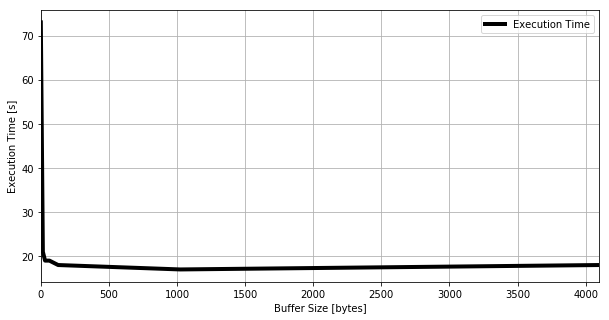
\includegraphics[width=\textwidth]{images/stressEquals}
    			\end{center}
    			\tab Como se puede observar, la gran distancia entre los valores iniciales (16, 32, ...) y el final (4096) hace que este
    			último gráfico no sea muy descriptivo. Por esta razón, mostraremos uno que toma los valores entre 1 y 128; ya que para
    			ese valor de buffer size, el tiempo ya se está estancado y podremos ver cómo varía de una mejor manera:
    			\begin{center}
		       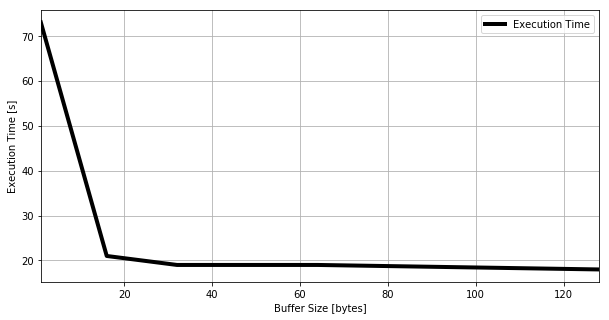
\includegraphics[width=\textwidth]{images/stressEqualsCloseUp}
    			\end{center}
    			\tab Vemos entonces que entre los primeros dos valores (1 y 16) hay un gran salto - más especificamente del $71\%$ - pero
    			a partir del próximo valor las diferencias ya son mínimas, siendo la máxima de dos segundos (entre 16 y 32). \\
    			\tab Finalmente, veremos los datos arrojados por los stress tests en los casos en que los buffers no tenían el mismo
    			tamaño. Para esto, se realizó un gráfico de barras en el que se muestra el tiempo de ejecución del programa para cada
    			par de tamaños de buffers (no se muestra tabla porque su extensión no permitiría observar correctamente los datos):
    			\begin{center}
		       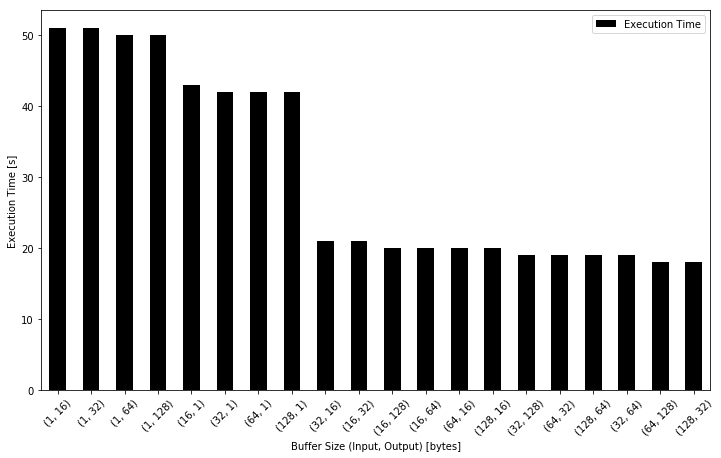
\includegraphics[width=\textwidth]{images/stressNonEquals}
    			\end{center}
    			\tab Este gráfico nos muestra datos interesantes y son los siguiente:
    			\begin{itemize}
    				\item En las primeras 8 columnas se puede observar que, en nuestro caso, es más importante tener un buffer de entrada
    				que de salida; pues cuando el buffer de entrada toma valor y el buffer de salida tiene tamaño 1 (que es lo mismo que
    				no tenerlo) los tiempos son mejores que en el caso inverso. De todas maneras, se debe decir que en las pruebas 
    				realizadas un poco menos de un cuarto de los caracteres que se leen se escriben, por lo que tiene sentido la
    				diferencia del aproximadamente $20\%$ que se observa (y si miramos el final del gráfico, el mejor resultado tiene
    				relación $\frac{o_{}size}{i_{}size} = \frac{1}{4}$ [aunque podría no significar nada]).
    				\item Una vez que ambos buffers son de más (o igual a) 16 bytes, el rendimiento es muy parecido en todos los casos.
    				\item No se puede decir que cuanto más grande es el buffer de entrada mejor es el rendimiento ni se puede establecer
    				una relación entre tamaños y rendimientos más que la mencionada en el primer item. Por ejemplo, la cupla (128, 64) es
    				peor que (64, 128) pero (128, 32) es mejor que esta última.
    			\end{itemize}

	\section{Conclusiones}
		Una conclusión importante obtenida de este trabajo es resultante de las pruebas de Stress; donde se puede ver que la lectura
		de archivos es una de las tareas más lentas que se pueden realizar pero que es muy fácil de resolver con el simple hecho de 
		realizar lecturas de más de un byte y almacenar la información en un buffer para luego acceder rápidamente, sin volver al 
		archivo. Por otro lado, también es importante destacar que esta mejora tiene un tope y no es 'cuanto más guardo más rápido
		va', sino que llega un punto (cierto tamaño de buffer) en que ya no se puede obtener mayor performance con este método.
\end{document}
